Para empezar a trabajar sobre la placa es necesario configurar las entradas y salidas para que se correspondan con las de la placa física.\\ 

Las salidas físicas para los \textbf{displays de 7 segmentos} se encuentran en los pines que se pueden ver en la siguiente tabla. Los displays se encuentran representados con el número 10 en la figura (\ref{fig:Spartan3TopSide}) del apartado (\ref{subsection:Spartan-3}).

Como se puede ver en la figura los 4 displays comparten 8 pines de control, para elegir un display u otro están los Ánodos de control, en la tabla (\ref{tab:anodoControl}).

\begin{table}[H]
        \centering
		\begin{tabular}{|c|c|c|c|c|c|c|c|c|}
			\hline
			\rowcolor[rgb]{0.21,0.69,0.87}\multicolumn{9}{|c|}{  \textbf{ {Salidas físicas Display 7 segmentos}}} \\
			\hline \hline
			\textbf{  Segmento  } & A & B & C & D & E & F & G & DP \\ 
			\hline
			\textbf{  FPGA Pin  }  & E14 & G13 & N15 & P15 & R16 & F13 & N16 & P16 \\ 
			\hline
			\multicolumn{9}{|c|}{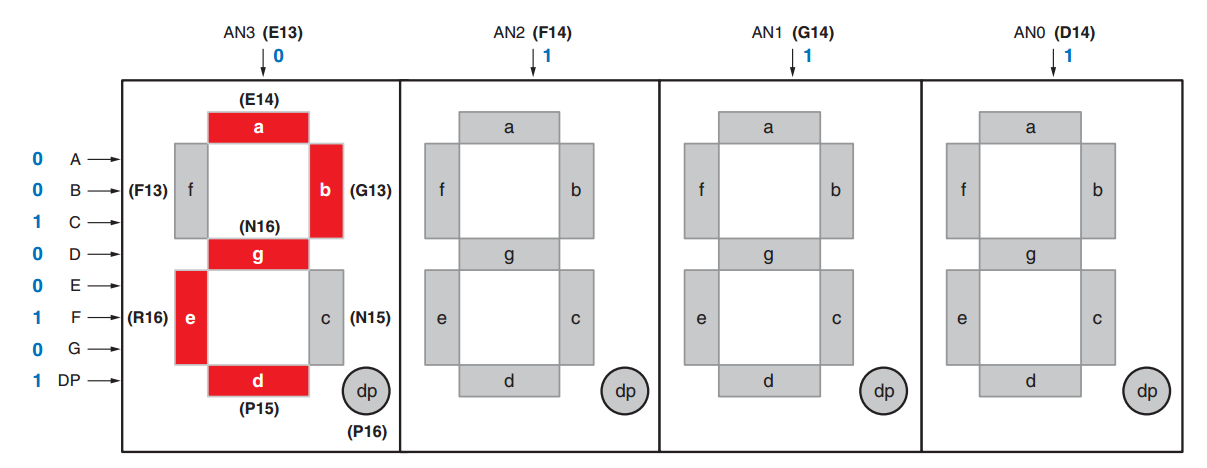
\includegraphics[width = 0.8\textwidth ]{Spartan3-7segment}}\\
			\hline
			 
		\end{tabular}
	\caption{ Salidas físicas de los displays en la Spartan-3 }
	\label{tab:tablaSalidas7Segmentos}
\end{table}

\begin{table}[H]
        \centering
		\begin{tabular}{|c|c|c|c|c|}
			\hline
			\rowcolor[rgb]{0.21,0.69,0.87}\multicolumn{5}{|c|}{  \textbf{ {Ánodos de control}}} \\
			\hline \hline
			\textbf{  Anodo Control  } & AN3 & AN2 & AN1 & AN0  \\
			\hline
			\textbf{  FPGA Pin  } & E13 & F14 & G14 & D14  \\
			\hline
			 
		\end{tabular}
	\caption{ Ánodos control (activos a nivel bajo) para los display de 7 segmentos }
	\label{tab:anodoControl}
\end{table}

Las entradas correspondientes a los \textbf{interruptores} se pueden ver en la siguiente tabla. Estos interruptores se encuentran representados con el número 11 en la figura (\ref{fig:Spartan3TopSide}) del apartado (\ref{subsection:Spartan-3}).

\begin{table}[H]
        \centering
		\begin{tabular}{|c|c|c|c|c|c|c|c|c|}
			\hline
			\rowcolor[rgb]{0.21,0.69,0.87}\multicolumn{9}{|c|}{  \textbf{ {Entradas Interruptores}}} \\
			\hline \hline
			\textbf{  Interruptor  } & SW7 & SW6 & SW5 & SW4 & SW3 & SW2 & SW1 & SW0 \\
			\hline
			\textbf{  FPGA Pin  } & K13 & K14 & J13 & J14 & H13 & H14 & G12 & F12 \\
			\hline
			 
		\end{tabular}
	\caption{ Entradas físicas de los interruptores en la Spartan-3 }
	\label{tab:tablaEntradasInterruptores}
\end{table}

Los pines de entrada correspondientes a los \textbf{pulsadores} se pueden ver en la siguiente tabla. Estos componentes se corresponden con los representados con el número 13 en la figura (\ref{fig:Spartan3TopSide}) del apartado (\ref{subsection:Spartan-3}).

\begin{table}[H]
        \centering
		\begin{tabular}{|c|c|c|c|c|}
			\hline
			\rowcolor[rgb]{0.21,0.69,0.87}\multicolumn{5}{|c|}{  \textbf{ {Entradas Pulsadores}}} \\
			\hline \hline
			\textbf{  Pulsador  } & BTN3 (Reset) & BTN2 & BTN1 & BTN0  \\
			\hline
			\textbf{  FPGA Pin  } & L14 & L13 & M14 & M13  \\
			\hline
			 
		\end{tabular}
	\caption{ Entradas físicas de los pulsadores en la Spartan-3 }
	\label{tab:tablaEntradasPulsadores}
\end{table}

Como se ha dicho en el apartado (\ref{subsection:Spartan-3}) la placa incorpora ocho LEDs, representados con el número 12 en la figura (\ref{fig:Spartan3TopSide}). A continuación se muestra la correlación de cada LED con la patilla de la FPGA:

\begin{table}[H]
        \centering
		\begin{tabular}{|c|c|c|c|c|c|c|c|c|}
			\hline
			\rowcolor[rgb]{0.21,0.69,0.87}\multicolumn{9}{|c|}{  \textbf{ {Salidas LED}}} \\
			\hline \hline
			\textbf{  LED  } & LD7 & LD6 & LD5 & LD4 & LD3 & LD2 & LD1 & LD0 \\
			\hline
			\textbf{  FPGA Pin  } & P11 & P12 & N12 & P13 & N14 & L12 & P14 & K12  \\
			\hline
			 
		\end{tabular}
	\caption{ Salidas físicas de los LEDs en la Spartan-3 }
	\label{tab:tablaSalidasLED}
\end{table}